\section{DIL\_\-AL\_\-List  Class Reference}
\label{classDIL__AL__List}\index{DIL_AL_List@{DIL\_\-AL\_\-List}}
{\tt \#include $<$dil2al.hh$>$}

Inheritance diagram for DIL\_\-AL\_\-List::\begin{figure}[H]
\begin{center}
\leavevmode
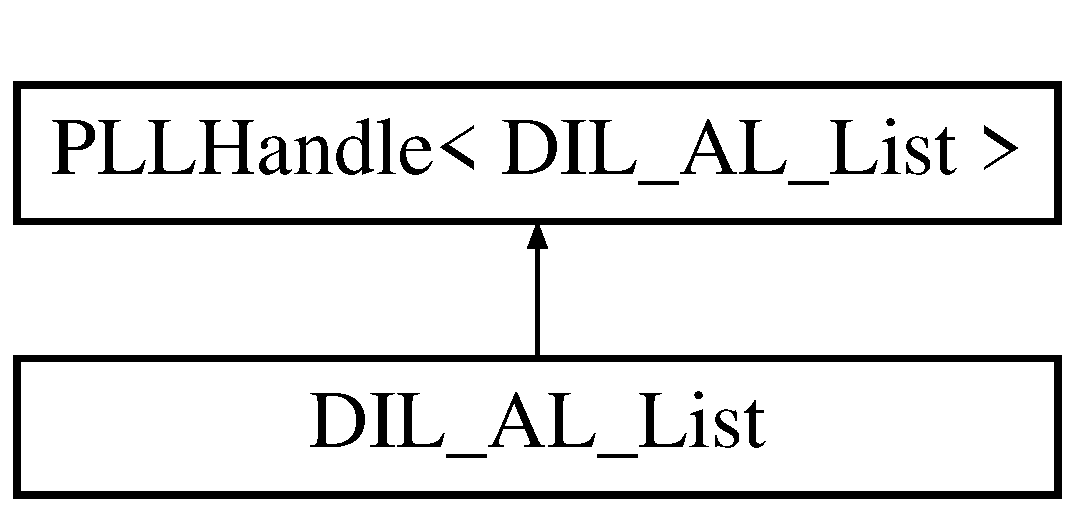
\includegraphics[height=2cm]{classDIL__AL__List}
\end{center}
\end{figure}
\subsection*{Public Methods}
\begin{CompactItemize}
\item 
{\bf DIL\_\-AL\_\-List} ({\bf DIL\_\-entry} \&e)
\item 
{\bf DIL\_\-AL\_\-List} ({\bf DIL\_\-entry} \&e, {\bf String} pfile, {\bf String} ptitle, float prelevance, float punbounded, float pbounded, time\_\-t ptargetdate, int ptdprop, float purgency, float ppriority)
\item 
{\bf $\sim$DIL\_\-AL\_\-List} ()
\item 
{\bf DIL\_\-entry} $\ast$ {\bf Superiorbyid} ()
\item 
bool {\bf Is\-Self\-Reference} ()
\item 
time\_\-t {\bf targetdate} ()
\item 
int {\bf tdproperty} ()
\item 
bool {\bf set\_\-targetdate} (time\_\-t td)
\item 
void {\bf set\_\-tdproperty} (int tdprop)
\item 
bool {\bf Write\_\-to\_\-Binary\_\-Cache} (ofstream \&cfl)
\item 
bool {\bf Read\_\-from\_\-Binary\_\-Cache} (ifstream \&cfl)
\item 
bool {\bf Binary\_\-Cache\_\-Diagnostic} (DIL\_\-AL\_\-List $\ast$cached, int \&testedbytes)
\end{CompactItemize}
\subsection*{Public Attributes}
\begin{CompactItemize}
\item 
{\bf filetitle\_\-t} {\bf al}
\item 
float {\bf relevance}
\item 
float {\bf unbounded}
\item 
float {\bf bounded}
\item 
float {\bf urgency}
\item 
float {\bf priority}
\end{CompactItemize}
\subsection*{Protected Attributes}
\begin{CompactItemize}
\item 
{\bf DIL\_\-entry} $\ast$ {\bf entry}
\item 
{\bf DIL\_\-entry} $\ast$ {\bf superior}
\item 
time\_\-t {\bf \_\-targetdate}
\item 
int {\bf \_\-tdproperty}
\end{CompactItemize}


\subsection{Constructor \& Destructor Documentation}
\index{DIL_AL_List@{DIL\_\-AL\_\-List}!DIL_AL_List@{DIL\_\-AL\_\-List}}
\index{DIL_AL_List@{DIL\_\-AL\_\-List}!DIL_AL_List@{DIL\_\-AL\_\-List}}
\subsubsection{\setlength{\rightskip}{0pt plus 5cm}DIL\_\-AL\_\-List::DIL\_\-AL\_\-List ({\bf DIL\_\-entry} \& {\em e})}\label{classDIL__AL__List_a0}




Definition at line 741 of file utilities.cc.

References DILSUPS\_\-BND\_\-UNSPECIFIED, DILSUPS\_\-PRI\_\-UNSPECIFIED, DILSUPS\_\-REL\_\-UNSPECIFIED, DILSUPS\_\-TD\_\-UNSPECIFIED, DILSUPS\_\-UNB\_\-UNSPECIFIED, and DILSUPS\_\-URG\_\-UNSPECIFIED.



\footnotesize\begin{verbatim}741                                      : entry(&e), superior(NULL), relevance(DILSUPS_REL_UNSPECIFIED),
742         unbounded(DILSUPS_UNB_UNSPECIFIED), bounded(DILSUPS_BND_UNSPECIFIED), _targetdate(DILSUPS_TD_UNSPECIFIED),
743         _tdproperty(0), urgency(DILSUPS_URG_UNSPECIFIED), priority(DILSUPS_PRI_UNSPECIFIED) {}
\end{verbatim}\normalsize 
\index{DIL_AL_List@{DIL\_\-AL\_\-List}!DIL_AL_List@{DIL\_\-AL\_\-List}}
\index{DIL_AL_List@{DIL\_\-AL\_\-List}!DIL_AL_List@{DIL\_\-AL\_\-List}}
\subsubsection{\setlength{\rightskip}{0pt plus 5cm}DIL\_\-AL\_\-List::DIL\_\-AL\_\-List ({\bf DIL\_\-entry} \& {\em e}, {\bf String} {\em pfile}, {\bf String} {\em ptitle}, float {\em prelevance}, float {\em punbounded}, float {\em pbounded}, time\_\-t {\em ptargetdate}, int {\em ptdprop}, float {\em purgency}, float {\em ppriority})}\label{classDIL__AL__List_a1}




Definition at line 745 of file utilities.cc.

References al, filetitle\_\-t::file, and filetitle\_\-t::title.



\footnotesize\begin{verbatim}745                                                                                                                                                                                         :
746                 entry(&e), superior(NULL), relevance(prelevance), unbounded(punbounded), bounded(pbounded), _targetdate(ptargetdate), _tdproperty(ptdprop), urgency(purgency), priority(ppriority) {
747         al.file = pfile;
748         al.title = ptitle;
749 }

\end{verbatim}\normalsize 
\index{DIL_AL_List@{DIL\_\-AL\_\-List}!~DIL_AL_List@{$\sim$DIL\_\-AL\_\-List}}
\index{~DIL_AL_List@{$\sim$DIL\_\-AL\_\-List}!DIL_AL_List@{DIL\_\-AL\_\-List}}
\subsubsection{\setlength{\rightskip}{0pt plus 5cm}DIL\_\-AL\_\-List::$\sim$DIL\_\-AL\_\-List ()\hspace{0.3cm}{\tt  [inline]}}\label{classDIL__AL__List_a2}




Definition at line 569 of file dil2al.hh.



\footnotesize\begin{verbatim}569 {} 
\end{verbatim}\normalsize 


\subsection{Member Function Documentation}
\index{DIL_AL_List@{DIL\_\-AL\_\-List}!Binary_Cache_Diagnostic@{Binary\_\-Cache\_\-Diagnostic}}
\index{Binary_Cache_Diagnostic@{Binary\_\-Cache\_\-Diagnostic}!DIL_AL_List@{DIL\_\-AL\_\-List}}
\subsubsection{\setlength{\rightskip}{0pt plus 5cm}bool DIL\_\-AL\_\-List::Binary\_\-Cache\_\-Diagnostic (DIL\_\-AL\_\-List $\ast$ {\em cached}, int \& {\em testedbytes})}\label{classDIL__AL__List_a11}




Definition at line 820 of file utilities.cc.

References \_\-targetdate, \_\-tdproperty, al, bounded, entry, filetitle\_\-t::file, priority, relevance, filetitle\_\-t::title, unbounded, urgency, and VOUT.

Referenced by DIL\_\-entry\_\-parameters::Binary\_\-Cache\_\-Diagnostic().



\footnotesize\begin{verbatim}820                                                                                  {
821   // test if the quick load cache process works reliably
822   // this is the original AL_List, cached is the one retrieved from the binary cache
823   //   start of this object test
824   int localtestedbytes = sizeof(PLLHandle<DIL_AL_List>) + sizeof(superior);
825   if ((*entry)!=(*(cached->entry))) VOUT << "*** DIL_AL_List entry mismatch\n"; // testing if DIL_ID==DIL_ID
826   localtestedbytes += sizeof(entry);
827   if (al.file!=cached->al.file) VOUT << "*** DIL_AL_List al.file mismatch\n";
828   if (al.title!=cached->al.title) VOUT << "*** DIL_AL_List al.title mismatch\n";
829   localtestedbytes += sizeof(al);
830   if (_targetdate!=cached->_targetdate) VOUT << "*** DIL_AL_List targetdate mismatch\n";
831   localtestedbytes += sizeof(_targetdate);
832   if (_tdproperty!=cached->_tdproperty) VOUT << "*** DIL_AL_List _tdproperty mismatch\n";
833   localtestedbytes += sizeof(_tdproperty);
834   if (relevance!=cached->relevance) VOUT << "*** DIL_AL_List relevance mismatch\n";
835   localtestedbytes += sizeof(relevance);
836   if (unbounded!=cached->unbounded) VOUT << "*** DIL_AL_List unbounded mismatch\n";
837   localtestedbytes += sizeof(unbounded);
838   if (bounded!=cached->bounded) VOUT << "*** DIL_AL_List hounded mismatch\n";
839   localtestedbytes += sizeof(bounded);
840   if (urgency!=cached->urgency) VOUT << "*** DIL_AL_List urgency mismatch\n";
841   localtestedbytes += sizeof(urgency);
842   if (priority!=cached->priority) VOUT << "*** DIL_AL_List priority mismatch\n";
843   localtestedbytes += sizeof(priority);
844   //   end of this object test
845   if (localtestedbytes!=sizeof(DIL_AL_List)) VOUT << "*** testedbytes!=sizeof(DIL_AL_List)\n";
846   testedbytes += localtestedbytes;
847   return true;
848 }
\end{verbatim}\normalsize 
\index{DIL_AL_List@{DIL\_\-AL\_\-List}!IsSelfReference@{IsSelfReference}}
\index{IsSelfReference@{IsSelfReference}!DIL_AL_List@{DIL\_\-AL\_\-List}}
\subsubsection{\setlength{\rightskip}{0pt plus 5cm}bool DIL\_\-AL\_\-List::Is\-Self\-Reference ()\hspace{0.3cm}{\tt  [inline]}}\label{classDIL__AL__List_a4}




Definition at line 1171 of file dil2al.hh.

References al, entry, DIL\_\-ID::str(), filetitle\_\-t::title, and DIL\_\-ID::valid().



\footnotesize\begin{verbatim}1171                                          {
1172         DIL_ID did(al.title);
1173         return ((entry->str()==al.title) || (!did.valid()));
1174 }
\end{verbatim}\normalsize 
\index{DIL_AL_List@{DIL\_\-AL\_\-List}!Read_from_Binary_Cache@{Read\_\-from\_\-Binary\_\-Cache}}
\index{Read_from_Binary_Cache@{Read\_\-from\_\-Binary\_\-Cache}!DIL_AL_List@{DIL\_\-AL\_\-List}}
\subsubsection{\setlength{\rightskip}{0pt plus 5cm}bool DIL\_\-AL\_\-List::Read\_\-from\_\-Binary\_\-Cache (ifstream \& {\em cfl})}\label{classDIL__AL__List_a10}




Definition at line 777 of file utilities.cc.

References \_\-targetdate, \_\-tdproperty, al, bounded, filetitle\_\-t::file, priority, READSOMETYPE, relevance, TEST\_\-LBUF\_\-BOUNDS, filetitle\_\-t::title, unbounded, urgency, and VOUT.

Referenced by DIL\_\-entry\_\-parameters::Read\_\-from\_\-Binary\_\-Cache().



\footnotesize\begin{verbatim}777                                                        {
778   const int LLEN = 1024;
779   char lbuf[LLEN];
780   // _targetdate
781   if ((cfl.read((READSOMETYPE) (&_targetdate), sizeof(_targetdate))).gcount()<sizeof(_targetdate)) return false;
782   // _tdproperty
783   if ((cfl.read((READSOMETYPE) (&_tdproperty), sizeof(_tdproperty))).gcount()<sizeof(_tdproperty)) return false;
784 #ifdef TEST_CACHE_READ
785   VOUT << "&&& _targetdate = " << _targetdate << ", _tdproperty = " << _tdproperty << '\n'; cout.flush();
786 #endif
787   // al.file
788   int alfilelen;
789   if ((cfl.read((READSOMETYPE) (&alfilelen), sizeof(alfilelen))).gcount()<sizeof(alfilelen)) return false;
790 #ifdef TEST_CACHE_READ
791   VOUT << "&&& alfilelen = " << alfilelen << '\n'; cout.flush();
792 #endif
793   TEST_LBUF_BOUNDS(alfilelen,"DIL_AL_List::Read_from_Binary_Cache()")
794   if ((cfl.read((READSOMETYPE) lbuf, alfilelen)).gcount()<alfilelen) return false;
795   lbuf[alfilelen]='\0';
796   al.file = lbuf;
797 #ifdef TEST_CACHE_READ
798   VOUT << "&&& al.file = " << al.file << '\n'; cout.flush();
799 #endif
800   // al.title
801   int altitlelen;
802   if ((cfl.read((READSOMETYPE) (&altitlelen), sizeof(altitlelen))).gcount()<sizeof(altitlelen)) return false;
803   TEST_LBUF_BOUNDS(altitlelen,"DIL_AL_List::Read_from_Binary_Cache()")
804   if ((cfl.read((READSOMETYPE) lbuf, altitlelen)).gcount()<altitlelen) return false;
805   lbuf[altitlelen]='\0';
806   al.title = lbuf;
807   // relevance
808   if ((cfl.read((READSOMETYPE) (&relevance), sizeof(relevance))).gcount()<sizeof(relevance)) return false;
809   // unbounded
810   if ((cfl.read((READSOMETYPE) (&unbounded), sizeof(unbounded))).gcount()<sizeof(unbounded)) return false;
811   // bounded
812   if ((cfl.read((READSOMETYPE) (&bounded), sizeof(bounded))).gcount()<sizeof(bounded)) return false;
813   // urgency
814   if ((cfl.read((READSOMETYPE) (&urgency), sizeof(urgency))).gcount()<sizeof(urgency)) return false;
815   // priority
816   if ((cfl.read((READSOMETYPE) (&priority), sizeof(priority))).gcount()<sizeof(priority)) return false;
817   return true;
818 }
\end{verbatim}\normalsize 
\index{DIL_AL_List@{DIL\_\-AL\_\-List}!set_targetdate@{set\_\-targetdate}}
\index{set_targetdate@{set\_\-targetdate}!DIL_AL_List@{DIL\_\-AL\_\-List}}
\subsubsection{\setlength{\rightskip}{0pt plus 5cm}bool DIL\_\-AL\_\-List::set\_\-targetdate (time\_\-t {\em td})\hspace{0.3cm}{\tt  [inline]}}\label{classDIL__AL__List_a7}




Definition at line 589 of file dil2al.hh.

References \_\-targetdate, \_\-tdproperty, and DILSUPS\_\-TDPROP\_\-FIXED.

Referenced by modify\_\-DIL\_\-group\_\-target\_\-dates().



\footnotesize\begin{verbatim}589 { if (_tdproperty==DILSUPS_TDPROP_FIXED) return false; _targetdate = td; return true; }
\end{verbatim}\normalsize 
\index{DIL_AL_List@{DIL\_\-AL\_\-List}!set_tdproperty@{set\_\-tdproperty}}
\index{set_tdproperty@{set\_\-tdproperty}!DIL_AL_List@{DIL\_\-AL\_\-List}}
\subsubsection{\setlength{\rightskip}{0pt plus 5cm}void DIL\_\-AL\_\-List::set\_\-tdproperty (int {\em tdprop})\hspace{0.3cm}{\tt  [inline]}}\label{classDIL__AL__List_a8}




Definition at line 590 of file dil2al.hh.

References \_\-tdproperty.



\footnotesize\begin{verbatim}590 { _tdproperty=tdprop; }
\end{verbatim}\normalsize 
\index{DIL_AL_List@{DIL\_\-AL\_\-List}!Superiorbyid@{Superiorbyid}}
\index{Superiorbyid@{Superiorbyid}!DIL_AL_List@{DIL\_\-AL\_\-List}}
\subsubsection{\setlength{\rightskip}{0pt plus 5cm}{\bf DIL\_\-entry} $\ast$ DIL\_\-AL\_\-List::Superiorbyid ()\hspace{0.3cm}{\tt  [inline]}}\label{classDIL__AL__List_a3}




Definition at line 1153 of file dil2al.hh.

References al, DIL\_\-entry::elbyid(), entry, PLLHandle$<$ DIL\_\-entry $>$::head(), superior, filetitle\_\-t::title, and DIL\_\-ID::valid().



\footnotesize\begin{verbatim}1153                                              {
1154 // assumes entry is in Detailed_Items_List
1155 // returns pointer to superior if found, pointer to self (*entry) if
1156 // no valid DIL ID was given, or NULL if the valid DIL ID could not
1157 // be found in the Detailed_Items_List
1158         if (!superior) { // fill the cache
1159                 DIL_ID did(al.title);
1160                 if (did.valid()) superior = entry->head()->elbyid(did);
1161                 else superior = entry;
1162         }
1163         return superior;
1164 }
\end{verbatim}\normalsize 
\index{DIL_AL_List@{DIL\_\-AL\_\-List}!targetdate@{targetdate}}
\index{targetdate@{targetdate}!DIL_AL_List@{DIL\_\-AL\_\-List}}
\subsubsection{\setlength{\rightskip}{0pt plus 5cm}time\_\-t DIL\_\-AL\_\-List::targetdate ()\hspace{0.3cm}{\tt  [inline]}}\label{classDIL__AL__List_a5}




Definition at line 587 of file dil2al.hh.

References \_\-targetdate.

Referenced by Detailed\_\-Items\_\-List::Get\_\-All\_\-DIL\_\-ID\_\-File\_\-Parameters(), and DIL\_\-entry::Local\_\-Target\_\-Date().



\footnotesize\begin{verbatim}587 { return _targetdate; }
\end{verbatim}\normalsize 
\index{DIL_AL_List@{DIL\_\-AL\_\-List}!tdproperty@{tdproperty}}
\index{tdproperty@{tdproperty}!DIL_AL_List@{DIL\_\-AL\_\-List}}
\subsubsection{\setlength{\rightskip}{0pt plus 5cm}int DIL\_\-AL\_\-List::tdproperty ()\hspace{0.3cm}{\tt  [inline]}}\label{classDIL__AL__List_a6}




Definition at line 588 of file dil2al.hh.

References \_\-tdproperty.



\footnotesize\begin{verbatim}588 { return _tdproperty; }
\end{verbatim}\normalsize 
\index{DIL_AL_List@{DIL\_\-AL\_\-List}!Write_to_Binary_Cache@{Write\_\-to\_\-Binary\_\-Cache}}
\index{Write_to_Binary_Cache@{Write\_\-to\_\-Binary\_\-Cache}!DIL_AL_List@{DIL\_\-AL\_\-List}}
\subsubsection{\setlength{\rightskip}{0pt plus 5cm}bool DIL\_\-AL\_\-List::Write\_\-to\_\-Binary\_\-Cache (ofstream \& {\em cfl})}\label{classDIL__AL__List_a9}




Definition at line 751 of file utilities.cc.

References \_\-targetdate, \_\-tdproperty, al, bounded, String::chars(), filetitle\_\-t::file, String::length(), priority, relevance, filetitle\_\-t::title, unbounded, and urgency.



\footnotesize\begin{verbatim}751                                                       {
752   // _targetdate
753   cfl.write((const void *) (&_targetdate), sizeof(_targetdate));
754   // _tdproperty
755   cfl.write((const void *) (&_tdproperty), sizeof(_tdproperty));
756   // al.file
757   int alfilelen = al.file.length();
758   cfl.write((const void *) (&alfilelen), sizeof(alfilelen));
759   cfl.write((const void *) al.file.chars(), alfilelen);
760   // al.title
761   int altitlelen = al.title.length();
762   cfl.write((const void *) (&altitlelen), sizeof(altitlelen));
763   cfl.write((const void *) al.title.chars(), altitlelen);
764   // relevance
765   cfl.write((const void *) (&relevance), sizeof(relevance));
766   // unbounded
767   cfl.write((const void *) (&unbounded), sizeof(unbounded));
768   // bounded
769   cfl.write((const void *) (&bounded), sizeof(bounded));
770   // urgency
771   cfl.write((const void *) (&urgency), sizeof(urgency));
772   // priority
773   cfl.write((const void *) (&priority), sizeof(priority));
774   return true;
775 }
\end{verbatim}\normalsize 


\subsection{Member Data Documentation}
\index{DIL_AL_List@{DIL\_\-AL\_\-List}!_targetdate@{\_\-targetdate}}
\index{_targetdate@{\_\-targetdate}!DIL_AL_List@{DIL\_\-AL\_\-List}}
\subsubsection{\setlength{\rightskip}{0pt plus 5cm}time\_\-t DIL\_\-AL\_\-List::\_\-targetdate\hspace{0.3cm}{\tt  [protected]}}\label{classDIL__AL__List_n2}




Definition at line 562 of file dil2al.hh.

Referenced by Binary\_\-Cache\_\-Diagnostic(), Read\_\-from\_\-Binary\_\-Cache(), set\_\-targetdate(), targetdate(), and Write\_\-to\_\-Binary\_\-Cache().\index{DIL_AL_List@{DIL\_\-AL\_\-List}!_tdproperty@{\_\-tdproperty}}
\index{_tdproperty@{\_\-tdproperty}!DIL_AL_List@{DIL\_\-AL\_\-List}}
\subsubsection{\setlength{\rightskip}{0pt plus 5cm}int DIL\_\-AL\_\-List::\_\-tdproperty\hspace{0.3cm}{\tt  [protected]}}\label{classDIL__AL__List_n3}




Definition at line 563 of file dil2al.hh.

Referenced by Binary\_\-Cache\_\-Diagnostic(), Read\_\-from\_\-Binary\_\-Cache(), set\_\-targetdate(), set\_\-tdproperty(), tdproperty(), and Write\_\-to\_\-Binary\_\-Cache().\index{DIL_AL_List@{DIL\_\-AL\_\-List}!al@{al}}
\index{al@{al}!DIL_AL_List@{DIL\_\-AL\_\-List}}
\subsubsection{\setlength{\rightskip}{0pt plus 5cm}{\bf filetitle\_\-t} DIL\_\-AL\_\-List::al}\label{classDIL__AL__List_m0}




Definition at line 571 of file dil2al.hh.

Referenced by Binary\_\-Cache\_\-Diagnostic(), DIL\_\-AL\_\-List(), Detailed\_\-Items\_\-List::Get\_\-All\_\-DIL\_\-ID\_\-File\_\-Parameters(), Is\-Self\-Reference(), modify\_\-DIL\_\-group\_\-target\_\-dates(), Read\_\-from\_\-Binary\_\-Cache(), Superiorbyid(), and Write\_\-to\_\-Binary\_\-Cache().\index{DIL_AL_List@{DIL\_\-AL\_\-List}!bounded@{bounded}}
\index{bounded@{bounded}!DIL_AL_List@{DIL\_\-AL\_\-List}}
\subsubsection{\setlength{\rightskip}{0pt plus 5cm}float DIL\_\-AL\_\-List::bounded}\label{classDIL__AL__List_m3}




Definition at line 581 of file dil2al.hh.

Referenced by Binary\_\-Cache\_\-Diagnostic(), Detailed\_\-Items\_\-List::Get\_\-All\_\-DIL\_\-ID\_\-File\_\-Parameters(), Read\_\-from\_\-Binary\_\-Cache(), and Write\_\-to\_\-Binary\_\-Cache().\index{DIL_AL_List@{DIL\_\-AL\_\-List}!entry@{entry}}
\index{entry@{entry}!DIL_AL_List@{DIL\_\-AL\_\-List}}
\subsubsection{\setlength{\rightskip}{0pt plus 5cm}{\bf DIL\_\-entry}$\ast$ DIL\_\-AL\_\-List::entry\hspace{0.3cm}{\tt  [protected]}}\label{classDIL__AL__List_n0}




Definition at line 560 of file dil2al.hh.

Referenced by Binary\_\-Cache\_\-Diagnostic(), Is\-Self\-Reference(), and Superiorbyid().\index{DIL_AL_List@{DIL\_\-AL\_\-List}!priority@{priority}}
\index{priority@{priority}!DIL_AL_List@{DIL\_\-AL\_\-List}}
\subsubsection{\setlength{\rightskip}{0pt plus 5cm}float DIL\_\-AL\_\-List::priority}\label{classDIL__AL__List_m5}




Definition at line 583 of file dil2al.hh.

Referenced by Binary\_\-Cache\_\-Diagnostic(), Detailed\_\-Items\_\-List::Get\_\-All\_\-DIL\_\-ID\_\-File\_\-Parameters(), Read\_\-from\_\-Binary\_\-Cache(), and Write\_\-to\_\-Binary\_\-Cache().\index{DIL_AL_List@{DIL\_\-AL\_\-List}!relevance@{relevance}}
\index{relevance@{relevance}!DIL_AL_List@{DIL\_\-AL\_\-List}}
\subsubsection{\setlength{\rightskip}{0pt plus 5cm}float DIL\_\-AL\_\-List::relevance}\label{classDIL__AL__List_m1}




Definition at line 578 of file dil2al.hh.

Referenced by Binary\_\-Cache\_\-Diagnostic(), Detailed\_\-Items\_\-List::Get\_\-All\_\-DIL\_\-ID\_\-File\_\-Parameters(), Read\_\-from\_\-Binary\_\-Cache(), and Write\_\-to\_\-Binary\_\-Cache().\index{DIL_AL_List@{DIL\_\-AL\_\-List}!superior@{superior}}
\index{superior@{superior}!DIL_AL_List@{DIL\_\-AL\_\-List}}
\subsubsection{\setlength{\rightskip}{0pt plus 5cm}{\bf DIL\_\-entry}$\ast$ DIL\_\-AL\_\-List::superior\hspace{0.3cm}{\tt  [protected]}}\label{classDIL__AL__List_n1}




Definition at line 561 of file dil2al.hh.

Referenced by Superiorbyid().\index{DIL_AL_List@{DIL\_\-AL\_\-List}!unbounded@{unbounded}}
\index{unbounded@{unbounded}!DIL_AL_List@{DIL\_\-AL\_\-List}}
\subsubsection{\setlength{\rightskip}{0pt plus 5cm}float DIL\_\-AL\_\-List::unbounded}\label{classDIL__AL__List_m2}




Definition at line 580 of file dil2al.hh.

Referenced by Binary\_\-Cache\_\-Diagnostic(), Detailed\_\-Items\_\-List::Get\_\-All\_\-DIL\_\-ID\_\-File\_\-Parameters(), Read\_\-from\_\-Binary\_\-Cache(), and Write\_\-to\_\-Binary\_\-Cache().\index{DIL_AL_List@{DIL\_\-AL\_\-List}!urgency@{urgency}}
\index{urgency@{urgency}!DIL_AL_List@{DIL\_\-AL\_\-List}}
\subsubsection{\setlength{\rightskip}{0pt plus 5cm}float DIL\_\-AL\_\-List::urgency}\label{classDIL__AL__List_m4}




Definition at line 582 of file dil2al.hh.

Referenced by Binary\_\-Cache\_\-Diagnostic(), Detailed\_\-Items\_\-List::Get\_\-All\_\-DIL\_\-ID\_\-File\_\-Parameters(), Read\_\-from\_\-Binary\_\-Cache(), and Write\_\-to\_\-Binary\_\-Cache().

The documentation for this class was generated from the following files:\begin{CompactItemize}
\item 
{\bf dil2al.hh}\item 
{\bf utilities.cc}\end{CompactItemize}
